\subsubsection[Algebra, Geometry, Lie Theory, Representation Theory]{Algebra, Geometry, Lie Theory, \\ Representation Theory}
\index{Penkov, Ivan}
\paragraph{Research Team}
Ivan Penkov (Professor)

\medskip

%\paragraph{General Description.}
Lie groups are continuous groups, i.e.\ manifolds with group structure,
and a Lie algebra is the tangent space of a Lie group at unity. The
structure theory of Lie algebras, developed by W. Killing, E. Cartan
and H. Weyl in the first half of the 20th century, belongs to the
jewels of modern mathematics. This theory is also a standard tool of
today's mathematical physics. A more recent fundamental achievement of
Lie theory is the complete description of a class of representations
of Lie groups and Lie algebras of fundamental importance. These are
the so called Harish Chandra modules, and their classification was
completed in the early 1980's by a tour de force using sophisticated
algebraic and geometric techniques.

\paragraph{Highlights}

Many deep problems in the structure theory of representations of Lie
algebras and Lie groups are still open. One such problem is the
classification of all simple modules $M$ over simple matrix Lie
algebras, satisfying the condition that $M$ decomposes as a direct sum
of finite dimensional isotypic components over a suitable
subalgebra. In the late 1990's my collaborators and I gave these
representations the name generalized Harish Chandra modules and
initiated a program to study them.

A main achievement of this program in recent years has been the
construction of large classes of new generalized Harish Chandra
modules, as well as the description of arbitrary reductive subalgebras
over which generalized Harish Chandra modules can have finite
dimensional isotypic components. In 2006 Vera Serganova and I have
obtained breakthrough results on bounded generalized Harish Chandra
modules. In particular, we have classified all such modules of a Lie
algebra of rank 2. The picture shows 4 ``smallest'' such modules of
$\mathfrak g=\mathrm{sp}(4)$. A paper is in progress.

\begin{figure}[ht]
  \begin{center}
    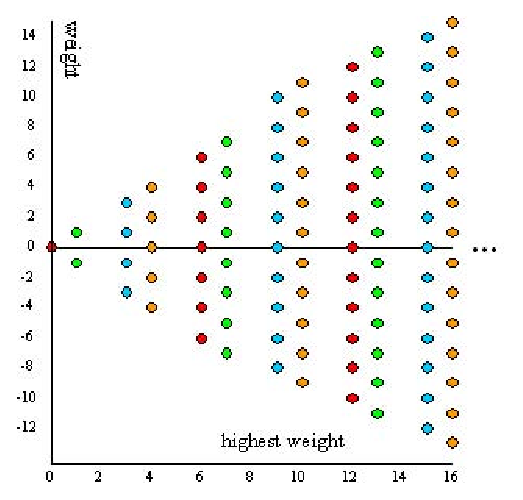
\includegraphics[width=\hsize]{Penkov/profPenkov_2006_fig1}
    \mycaption{Four multiplicity free
    $(\mathrm{sp}(4),\mathrm{sl}(2))$-modules pictured in different
    colors: each module is the direct sum of the
    $\mathrm{sl}(2)$-strings of the corresponding color. Note that
    there is no module with an $\mathrm{sl}(2)$-string of length
    3.}\label{fig:profPenkov}
   \end{center}
\end{figure}

Another program, in which I am actively working, is the structure
theory of the classical locally finite Lie algebras. The distant goal
of my collaborators and myself is to develop a structure theory which
would have the same detail as the classical structure theory of finite
dimensional Lie algebras. Notable successes in the recent years have
been a complete description of Cartan and Borel subalgebras, the
construction of a theory of weight modules, and an infinite
dimensional version of the Borel-Weil-Bott theorem for root-reductive
ind-groups. These results are based on innovative infinite dimensional
techniques such as generalized flags and their corresponding
homogeneous ind-spaces. In 2006, I. Dimitrov and I have completed the
solution of a difficult open problem: we have constructed a
Bott-Borel-Weil theory for diagonal ind-groups. A paper is in
progress.

Finally, I am pursuing a program in infinite dimensional algebraic
geometry. More specifically, I am studying vector bundles on
homogeneous ind-spaces. In 2006, A. Tikhomirov and I have completed
our work on vector bundles of rank 2 on twisted ind-grassmanians and
have made a breakthrough in the study of vector bundles of arbitrary
rank on twisted ind-grassmanians: we have proved a general conjecture
of mine in the so called ``tame'' case. A paper is in progress.


\paragraph{Organization}
\begin{enumerate}
\item Research in Pairs at the {\sl Mathematisches Forshungsinstitut Oberwolfach,} July 2006.
\item Workshop {\em Generalized Harish Chandra modules of $\mathrm{gl}(\infty)$,} Banff International Reseach Station, Canada, August--September 2006.
\end{enumerate}

\paragraph{Collaborations}
\begin{enumerate}
\item {\sl University of California at Berkeley, USA} \\ 
  Prof.~V. Serganova \\
  Generalized Harish Chandra modules
\item {\sl University of California at Berkeley, USA} \\
  Graduate students E. Dan-Cohen and N. Snyder \\
  Cartan subalgebras of root-reductive Lie algebras
\item {\sl Yale University, USA} \\
  Prof.~G. Zuckerman \\
  Generalized Harish Chandra Modules
\item {\sl Queens University, Canada} \\
  Prof.~I. Dimitrov \\
  Infinite dimensional representation theory and geometry
\item {\sl Yaroslavl University, Russia} \\
  Prof.~A. Tikhomirov \\
  Vector bundles on homogeneous ind-spaces
\item {\sl University of California at Berkeley, USA} \\
  Prof.~J. Wolf \\
  Generalized Harish Chandra modules of $\mathrm{gl}(\infty)$
\end{enumerate}

\paragraph{Grants}
\begin{enumerate}
\item
Separate grants for the workshops described above.
\end{enumerate}
\nocite{Penkov1key}
\nocite{Penkov2key}
